\documentclass{article}

\usepackage{a4wide}
\usepackage[utf8]{inputenc}
\usepackage[T1]{fontenc}
\usepackage[french]{babel}
\usepackage[babel=true]{csquotes} % guillemets français
\usepackage[export]{adjustbox}% http://ctan.org/pkg/adjustbox
\usepackage{graphicx}
\graphicspath{{image/}}
\usepackage{color}
\usepackage{hyperref}
\usepackage[section]{placeins}
\hypersetup{colorlinks,linkcolor=,urlcolor=blue}

\usepackage{amsmath}
\usepackage{amssymb}

\usepackage{subcaption}

\title{Rapport de Développement mobile \\[0.2em]\smaller{} En route vers Namek}

\author{Mehdi Bouchet\\L3 Informatique}

\begin{document}

\maketitle
\begin{abstract}
\textbf{En route vers Namek} est un jeu mobile développé par Mehdi Bouchet.\\Le principe est simple. Le joueur doit exterminer les astéroides qui foncent droit sur son vaisseau en cliquant sur celui-ci afin d'accéder à la planète Namek tant convoitée par les humains.
\end{abstract}

\section{Introduction}
\subsection{Cadre du jeu}
Les humains ayant découverts l'existence d'une planète remplie d'or qu'ils finiront par nommer Planète Namek, projètent d'y faire un tour. Mais le chemin qui y mène est rude ! Celui-ci est rempli d'astéroides à tout bord. Les humains ont donc crée une technologie appelé K-12, un rayon laser permettant de pouvoir exterminer tout les astéroides de leur passage. Vous avez été choisi pour porter la lourde responsabilité de manier ce nouvel objet. C'est l'heure de l'embarcation à bord du vaisseau. À vous de jouer.

\section{Vue d'ensemble}
\subsection{Activités}
Le jeu est composé de 3 activités

\subsubsection{MainMenuActivity}
Cette activité est lançée automatiquement lors du lancement du jeu.

\paragraph{Roles}C'est elle qui s'occupe de l'affichage du menu principal.
\paragraph{Architecture}On y retrouve 2 boutons: Start et Highscore tout deux centrés au milieu. Au clic sur l'un des boutons, l'activité va changer d'activité en fonction du boutons pressé. Start appelle l'activité IngameActivity et Highscore l'activité HighscoreActivity.

\begin{figure}
\centering
 \begin{subfigure}[b]{0.4\textwidth}
  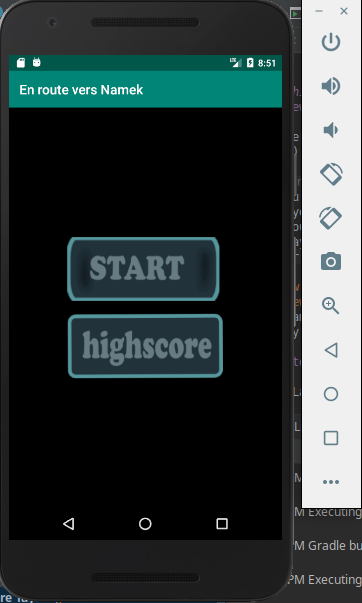
\includegraphics[width=\textwidth]{images/mainMenuView.png}
  \caption{Activité MainMenuActivity}
 \end{subfigure}
\end{figure}

\vspace{1\baselineskip}

\subsubsection{IngameActivity}
Cette activité est l'activité majeure de l'application.

\paragraph{Roles}: C'est elle qui s'occupe de l'affichage du menu principal.
\paragraph{Architecture}: La methode \textit{onCreate}, l'activité initialise la partie et ses paramètres associés. On y retrouve donc l'objet le plus important qui est de type \textbf{Partie} qui représente la partie lancée. Par la même occasion, l'activité initialise la base de donnée, qui prend forme d'un Adapter, l'objet de type \textbf{AlertDialog.Builder} qui permettra l'interaction avec l'utilisateur qui s'effectuera en fin de partie, llors de la saisie du nom du joueur mais encore, elle met en place les Listeners qui vont "écouter" sur les boutons d'interactions avec l'utilisateur en fin de partie.

\begin{figure}
\centering
 \begin{subfigure}[b]{0.4\textwidth}
  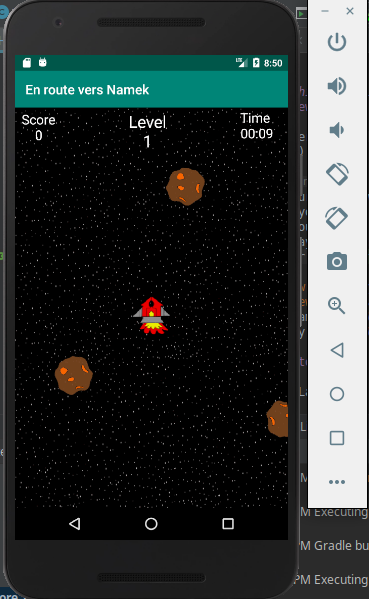
\includegraphics[width=\textwidth]{images/ingameView.png}
  \caption{Activité IngameActivity}
 \end{subfigure}
\end{figure}

\subsubsection{HighscoreActivity}
\paragraph{Roles}: Cette activité permet d'afficher les meilleurs scores enregistrés dans la base de données.
\paragraph{Architecture}: Elle est composée d'une listView permettant d'afficher la liste des meilleurs scores enregistrés. Un bouton Play again y est affiché juste en dessous.
\paragraph{Fonctionnement}: Elle ouvre une connexion avec la base de données, récupère les meilleurs scores grâce à l'adaptateur \textbf{HighscoreAdapter} puis les affiche sous forme de liste.
\paragraph{}Cette liste est issue de l'adapteur HighscoreAdapter qui va, de part sa méthode getView, formater l'affichage de la liste des Highscores qui lui a été fournie, afin de les rendre plus lisible à l'écran.
Il y est ajouté aussi la fonctionnalité de suppression du score associé à un nom du joueur lors de l'appui de l'astéroide précédant celui ci.

\begin{figure}
\centering
 \begin{subfigure}[b]{0.4\textwidth}
  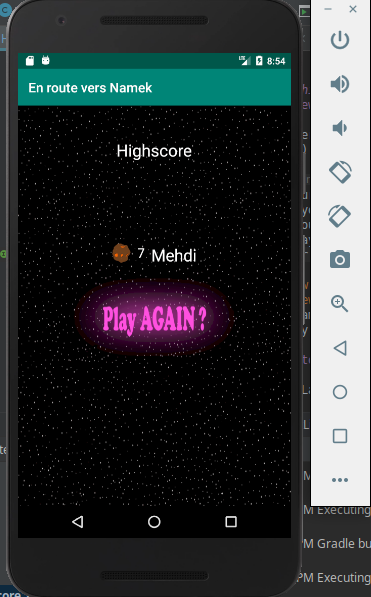
\includegraphics[width=\textwidth]{images/highscoreView.png}
  \caption{Activité HighscoreActivity}
 \end{subfigure}
\end{figure}


\subsection{Les classes}
Plusieurs classes ont été utilisés afin de pouvoir réaliser ce jeu.

\subsubsection{ObjectView}
Cette classe héritant de la classe View permet de représenter un objet dans une partie. Elle est caractérisé par sa position, sa taille, son image de fond et la partie auquelle elle est associée.
Une méthode interessante dans \textit{hasCollision}(ObjectView m) permettant de déterminer si un objet m est rentré en collision avec le ObjectView considéré.

Il y a deux types d'ObjectView, le VaisseauView et le MeteoreView.
\begin{itemize}
    \item "VaisseauView" étant la vue du vaisseau
    \item "MeteoreView" étant la vue d'un météore
\end{itemize}
\begin{figure}
\centering
 \begin{subfigure}[b]{0.4\textwidth}
  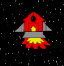
\includegraphics[width=\textwidth]{images/vaisseauView.png}
  \caption{Vue VaisseauView}
 \end{subfigure}
  \begin{subfigure}[b]{0.4\textwidth}
  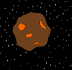
\includegraphics[width=\textwidth]{images/meteoreView.png}
  \caption{Vue MeteoreView}
 \end{subfigure}
\end{figure}

\subsubsection{VaisseauView}
MeteoreView est une ObjectView avec comme image de fond, un meteore.
\subsubsection{MeteoreView}
\textbf{MeteoreView} est donc une ObjectView un peu particulier de part son usage récurrent dans chaque partie. En effet chaque MeteoreView doivent respecter certaines conditions \\
Elles doivent être générer à l'exterieur de l'écran, elle doit bouger et réagir à au clic du joueur.

\paragraph{Generation}
Cette vue doit être générée en dehors de l'écran pour donner l'effet qu'il arrive de loin. Ceci est fait par le code suivant
\begin{verbatim}
        do
            generatePosition();
        while(g.hasCollision(this));
\end{verbatim}

\textit{generatePosition}() va générer une position aléatoire a l'extérieur de la zone vue par l'utilisateur. \\
Pour éviter que deux météores soient générés au même endroit au même moment, la vue prend la précaution de vérifier si il n'y a pas une collision avec un autre météore grâce à la méthode \textit{hasCollision}(ObjectView v) de l'objet g de type Partie

\paragraph{Mouvement}
L'effet de mouvement du temps t au temps t+1 est géré par la méthode \textit{updatePosition}() qui va déterminer la future position du météore. Etant donné que les météores convergent vers le vaisseau, que l'on a la position du vaisseau (grâce à partie.vaisseau) et du météore en question, une simple manipulation mathématique des vecteurs permet de calculer les prochaines coordonnées. \\
A noté que l'on régule la vitesse des météores en multipliant la prochaine position par un coefficient speed (qui est un attribut du meteore).

\paragraph{Listeners}
Une fois générer et visible a l'écran, le météore est cliquable. L'utilisateur doit pouvoir détruire le météore à l'appui sur ce dernier. \\
Cette fonctionnalité est faite par l'usage d'un Listener \textbf{onClickListener} que l'on implemente à cette classe. Il va permettre d'écouter le moment où l'utilisateur clique sur le météore. Au clic de l'utilisateur, la methode onClick sera executée. Comme indiqué ci-dessous, onClick appelera \textit{clearAnimation}() qui permettra de supprimer l'effet de rotation du météore, et \textit{partie.onClickMeteore(Meteore m)} qui va permettre la destruction du météore en mémoire par la partie qui lui est associée.
\begin{verbatim}
        final Meteores met= this;
        this.setOnClickListener(new OnClickListener() {
            @Override
            public void onClick(View v) { clearAnimation(); partie.onClickMeteore(met); }
        });
\end{verbatim}

\subsubsection{Partie}
Cette classe va permettre la représentation d'une partie dans la mémoire.\\
Dans son constructeur, tout les parametres necessaires sont initialisés: Le tableau de météores représentant l'ensemble des météores en jeu, le Handler pour pouvoir gérer le séquencage des actions et modifications d'états de la partie, le niveau du joueur, son score ect.. \\
L'activité inGameActivity démarre le jeu une fois initialiser grâce à la méthode \textit{startGame}() que possède Partie qui va:
\begin{itemize}
    \item afficher les vues necessaires
    \item générer une instance de MeteoresWaveManager permettant la \item gestion des vagues de météore (appel de runMeteoresManager qui execute le manager toutes les 10ms)
\begin{verbatim}
    private void runMeteoresManager() {
        MeteoresTasks metTask= new MeteoresTasks(this, handler);
        timer.scheduleAtFixedRate(metTask, 0, 10);
    }
\end{verbatim}
    \item générer un gestionnaire de position qui va permettre de mettre a jour la position des météores en jeu et la vérification de l'état du jeu. (appel de \textbf{runUpdateManager} qui execute le manager toutes les 10ms) C'est dans ce manager que va être géré la collision avec le vaisseau et va donc gérer l'état du jeu.
    \item Demarrer le chrono et changer l'état du jeu qui est géré par l'attribut state.
\end{itemize}

\subsection{Points interessants}
\subsubsection{Gestion des niveaux}
\paragraph{} La gestion des niveaux se fait en fonction du score que l'on obtient en détruisant des météores. A chaque appel de la méthode onClickMeteore(Meteore m), on vérifie si la partie doit s'intensifier ou pas via l'appel de la méthode \textit{updateLevel}() qui va faire le nécessaire. Plus le joueur détruit de météore, plus le niveau augmente. De plus, l'état des objets dépend du niveau. \\
\textit{Exemple: la rotation et la vitesse de déplacement d'un météore dépend du niveau. Le choix des pauses entre les vagues, du durée des vagues et de la difficulté des vagues se déterminent aussi en fonction du niveau de jeu. }

\paragraph{}Plusieurs méthodes ont été crée dans le but de déterminer ces parametres là en fonction du niveau.
\begin{itemize}
    \item getMaxMeteore détermine le nombre de météores maximal que peut contenir une vague.
    \item getChoice   détermine la plage des types de vagues autorisée (Niveau 1, il n'y a que la vague continue qui est en marche)
    \item getWaveDuration détermine la durée d'une vague.
    \item getRotateMs détermine le temps que met une météore pour tourner autour d'elle même
\end{itemize}

\subsubsection{Fin du jeu}
\paragraph{} A la fin d'une partie, il est proposé au joueur d'enregistrer son score ou pas dans une base de données. Cette fonctionnalité est disponible grâce aux Adapter.

\begin{verbatim}
    public void showEndGameModal(){
        builder.setMessage(R.string.saveScore).setPositiveButton(R.string.yes, confirmHSListener)
                .setNegativeButton(R.string.no, confirmHSListener).show();
    }
\end{verbatim}
    Affichage de la fenetre Modale demandant au joueur s'il souhaite enregistrer ou non son score.
    

\paragraph{}
Cette fonction est appelé lors de la collision entre le vaisseau et un meteore. Elle permet de définir une fenetre modale demandant au joueur s'il souhaite enregistrer son score. On attache aux deux boutons un Listener (nommé \textbf{confirmHSListener}) qui va afficher ou non une autre fenetre modale permettant au joueur de rentrer son nom. (voir ci dessous)
\begin{figure}
\centering
 \begin{subfigure}[b]{0.4\textwidth}
  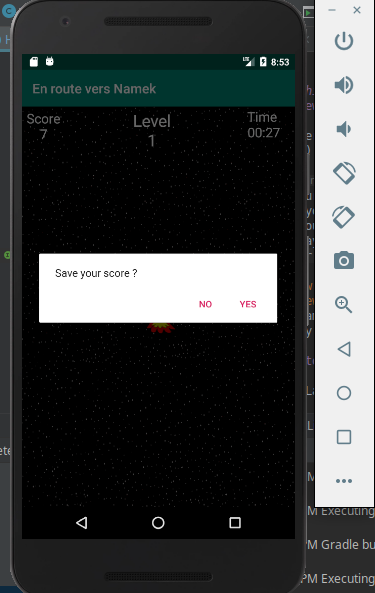
\includegraphics[width=\textwidth]{images/saveScore1.png}
  \caption{Modal affichée lors de la fin de partie}
 \end{subfigure}
\end{figure}

\begin{verbatim}
    private void showSaveNameModal(){
        builder.setMessage(getString(R.string.saveName))
                .setPositiveButton(R.string.save,saveHSListener)
                .setNegativeButton(R.string.cancel, saveHSListener);

        namePlayer = new EditText(mContext);
        LinearLayout.LayoutParams lp = new LinearLayout.LayoutParams(
                LinearLayout.LayoutParams.MATCH_PARENT,
                LinearLayout.LayoutParams.MATCH_PARENT);
        namePlayer.setLayoutParams(lp);
        builder.setView(namePlayer);

        builder.show();
    }
\end{verbatim}
On ajoute le bouton namePlayer à a fenetre modale créer grâce à builder.


\subsubsection{Persistance des données}
\paragraph{}
A la fin d'une partie, il est proposé au joueur d'enregistrer son score ou pas dans une base de données. Cette fonctionnalité est disponible grâce aux Adapter.

\paragraph{}
Cette classe va permettre la gestion de la base de donnée.
En créant une instance de cette classe, n'importe quelle classe pourra communiquer avec la base de donnée. IngameActivity l'utilise lors de l'enregistrement du score du joueur.
\begin{verbatim}
    public ArrayList<Highscore> getBestHighscore(int nb){
        ArrayList<Highscore> Highscores = new ArrayList<>();
        Cursor c =  mDB.query(HIGHSCORE_TABLE_NAME,
                new String[] {HIGHSCORE_COL_ID, HIGHSCORE_COL_NAME, HIGHSCORE_COL_SCORE},
                null,
                null,
                null,
                null,
                HIGHSCORE_COL_SCORE+" desc", Integer.toString(nb) );
        c.moveToFirst();
        while(!c.isAfterLast()){
            Highscores.add( new Highscore(
                            c.getInt(0),
                            c.getString(1),
                            c.getInt(2)
                    )
            );
            c.moveToNext();
        }
        return Highscores;
    }
    \end{verbatim}
Cette méthode permet de récuperer nb meilleurs scores enregistrés dans la base de donnée. mDB étant la base de donnée manipulée, on effectue une requête (query) permettant de récupérer les nb meilleurs scores qui sont stockés dans un Cursor c. Cette requête est équivalente en SQL à "SELECT HIGHSCORE\_COL\_ID, HIGHSCORE\_COL\_NAME, HIGHSCORE\_COL\_SCORE FROM HIGHSCORE\_TABLE\_NAME ORDER BY HIGHSCORE\_COL\_SCORE LIMIT nb" )
On effectue une itération sur les objets contenue dans Cursor afin de produire des objets de type Highscore. On retourne enfin le tableau des nb Highscore.

\subsection{Point Délicat}
\subsubsection{MeteoresWaveManager}
\parabraph{}Cette classe héritant de la classe java.util.TimerTask est une classe représentant un gestionnaire de vague (ou tache) de météore.
\parabraph{}C'est la classe la plus délicate du jeu mais c'est aussi le cerveau de l'application. En effet, elle est utilisée pour la gestion du mouvement perpétuelle des météores, le choix d'utiliser un gestionnaire de tache me semblait intéressant afin de pouvoir paralléliser la gestion de la partie avec de la gestion des vagues de météores et de leurs états (Collision, Position ect). 

\parabraph{}Cette classe est définie par le choix du type de la vague (attribut choiceTask ) en cours du temps que la tache en cours va prendre ( attribut ms) et du nombre de météore que va devoir générer la tache en ms seconde ( nbMeteores ).

\parabraph{}On intialise cette classe en lui attribuant un type de vague aléatoire. 

3 choix sont possibles: 

\paragraph{Vague continue}nbMeteores est envoyé en direction du vaisseau à intervalles réguliers en ms secondes.
\paragraph{Vague Instantannée}nbMeteores est envoyé en direction du vaisseau instantannément.
\paragraph{Vague aleatoire}nbMeteores est envoyé en direction du vaisseau suivant l'un des deux types de vagues précédent.

\paragraph{}
Le \textbf{MeteoresWaveManager} doit être appelé assez régulierement pour pouvoir mettre à jour l'état de la vague, et l'état dépend de certains attributs de la partie associée. Voilà pourquoi on utilise un objet de type Handler généré au début de la partie en cours qui va permettre de séquencer toutes les actions faites durant la partie afin qu'il n'y ait pas de données communes à chaque classe qui soit modifiées au même instant t dans la partie (Progammation concurrente).

\subsection{Amélioration}
\begin{itemize}
    \item Enregistrement du score (factoriser la connexion à la base de donnée, utilisation de putExtra lors de l'intent vers HighscoreActivity pour ne faire qu'une ouverture de base de donnée)
    \item Mouvement du vaisseau
    \item Mouvement sinusoidale des meteores
    \item Difficulté des niveaux à ajuste
\end{itemize}

\bibliographystyle{plain}
\bibliography{rapport}

\nocite{*}
\end{document}